% ======================================================================
% TECHNICAL_PRESENTATION.tex
% Recorded technical walkthrough of the project (screen-record narration).
% Autonomous TEC Atmospheric-Water-Harvesting PV-Cleaning Robot
% Rahma El-Hamouly -- REE598 Graduation Project
% Build: pdflatex TECHNICAL_PRESENTATION.tex  (run twice)
% Shares the look of DEFENSE_PRESENTATION.tex via tex/nac_beamer_theme.tex
% ======================================================================
\documentclass[aspectratio=169,10pt]{beamer}

% Shared modern NAC theme (palette, frame titles, footline, dividers).
% ======================================================================
% nac_beamer_theme.tex  --  shared modern Beamer styling for the
% TEC PV-cleaning-robot decks (defense + technical recording).
% pdflatex-safe: no external fonts, no metropolis dependency.
% Build each deck with: pdflatex <deck>.tex  (run twice for the
% progress bar and section references).
% ======================================================================

\usetheme{default}
\useinnertheme{rectangles}
\setbeamertemplate{navigation symbols}{}
\setbeamercovered{transparent}

% --- packages (shared by both decks) ---
\usepackage[utf8]{inputenc}
\usepackage[T1]{fontenc}
\usepackage{lmodern}
\usepackage{xcolor}
\usepackage{tikz}
\usetikzlibrary{calc}
\usepackage{siunitx}
\usepackage{graphicx}
\usepackage{booktabs}
\usepackage{amsmath}

% --- siunitx custom units (shared) ---
\DeclareSIUnit{\Wp}{Wp}
\DeclareSIUnit{\kWp}{kWp}
\DeclareSIUnit{\Wh}{Wh}
\DeclareSIUnit{\kWh}{kWh}
\DeclareSIUnit{\EGP}{EGP}
\DeclareSIUnit{\year}{yr}
\sisetup{detect-weight=true,detect-family=true}

% --- palette (NAC navy / water teal / solar sand) ---
\definecolor{nacblue}{RGB}{20,52,84}
\definecolor{nacblueL}{RGB}{37,86,128}
\definecolor{nacteal}{RGB}{0,150,158}
\definecolor{nacsand}{RGB}{226,170,74}
\definecolor{nacink}{RGB}{31,36,42}
\definecolor{nacgray}{RGB}{108,118,128}
\definecolor{naclight}{RGB}{244,247,250}

% --- base colours ---
\setbeamercolor{normal text}{fg=nacink,bg=white}
\setbeamercolor{alerted text}{fg=nacteal}
\setbeamercolor{structure}{fg=nacblue}
\setbeamercolor{title}{fg=nacblue}
\setbeamercolor{frametitle}{fg=nacblue,bg=white}
\setbeamercolor{itemize item}{fg=nacteal}
\setbeamercolor{itemize subitem}{fg=nacsand}
\setbeamercolor{itemize subsubitem}{fg=nacblueL}
\setbeamercolor{enumerate item}{fg=nacblue}
\setbeamercolor{block title}{fg=white,bg=nacblue}
\setbeamercolor{block body}{fg=nacink,bg=naclight}
\setbeamercolor{caption name}{fg=nacgray}

% --- fonts ---
\setbeamerfont{title}{series=\bfseries,size=\LARGE}
\setbeamerfont{frametitle}{series=\bfseries,size=\large}
\setbeamerfont{block title}{series=\bfseries,size=\normalsize}
\setbeamerfont{author in head/foot}{size=\scriptsize}
\setbeamerfont{title in head/foot}{size=\scriptsize}
\setbeamerfont{date in head/foot}{size=\scriptsize}

% --- blocks: flat, rounded, no shadow ---
\setbeamertemplate{blocks}[rounded][shadow=false]
\setbeamertemplate{itemize items}[circle]
\setbeamertemplate{caption}[numbered]
\setbeamertemplate{frametitle continuation}{}
\setlength{\leftmargini}{1.4em}

% --- frame title with a teal accent rule underneath ---
\setbeamertemplate{frametitle}{%
  \nointerlineskip%
  \vskip0.55em%
  \begin{beamercolorbox}[wd=\paperwidth,sep=0pt,leftskip=0.55cm,rightskip=0.55cm]{frametitle}%
    {\usebeamerfont{frametitle}\usebeamercolor[fg]{frametitle}\insertframetitle\strut\par}%
    \vskip3pt%
    {\color{nacteal}\rule{2.4cm}{2.2pt}}%
  \end{beamercolorbox}%
  \vskip0.35em%
}

% --- minimal footline with a teal progress bar ---
\setbeamertemplate{footline}{%
  \pgfmathsetmacro{\nacprog}{\insertframenumber/(\inserttotalframenumber<1?1:\inserttotalframenumber)}%
  \hbox to\paperwidth{%
    \rlap{\color{nacblue!12}\rule{\paperwidth}{1.6pt}}%
    \rlap{\color{nacteal}\rule{\nacprog\paperwidth}{1.6pt}}\hfil}%
  \vskip2pt%
  \hbox to\paperwidth{%
    \hskip0.45cm{\color{nacgray}\usebeamerfont{author in head/foot}\insertshortauthor}\hfil
    {\color{nacgray}\usebeamerfont{title in head/foot}\insertshorttitle}\hfil
    {\color{nacblue}\usebeamerfont{date in head/foot}\insertframenumber\,/\,\inserttotalframenumber}\hskip0.45cm}%
  \vskip3pt%
}

% --- section divider slides ---
\AtBeginSection[]{%
  {\setbeamertemplate{footline}{}%
   \begin{frame}[plain,noframenumbering]%
    \begin{tikzpicture}[remember picture,overlay]%
      \fill[nacblue](current page.south west)rectangle(current page.north east);%
      \fill[nacteal](current page.south west)rectangle([yshift=6pt]current page.south east);%
    \end{tikzpicture}%
    \vfill
    \begin{center}
      {\color{nacsand}\large\bfseries Part~\insertsectionnumber}\\[0.55em]
      {\color{white}\Huge\bfseries\insertsection}\\[0.75em]
      {\color{nacteal}\rule{3cm}{2.5pt}}
    \end{center}
    \vfill
   \end{frame}}%
}

% --- reusable custom title slide: \nactitleframe ---
\newcommand{\nactitleframe}[5]{%
  % #1 eyebrow line, #2 title (may use \\), #3 subtitle, #4 author, #5 footer line
  {\setbeamertemplate{footline}{}%
   \begin{frame}[plain,noframenumbering]%
    \begin{tikzpicture}[remember picture,overlay]%
      \fill[nacblue](current page.south west)rectangle(current page.north east);%
      \fill[nacteal](current page.south west)rectangle([yshift=7pt]current page.south east);%
    \end{tikzpicture}%
    \vfill
    \begin{center}
      {\color{nacsand}\large\bfseries #1}\\[1.05em]
      {\color{white}\usebeamerfont{title}#2}\\[0.8em]
      {\color{nacteal}\rule{4cm}{2.5pt}}\\[0.8em]
      {\color{white!88}\large #3}\\[1.7em]
      {\color{white}\large\bfseries #4}\\[0.35em]
      {\color{white!75}\normalsize #5}
    \end{center}
    \vfill
   \end{frame}}%
}


\graphicspath{{figures/}{figures/slides/}}

% --- title metadata (used by the footline) ---
\title[Self-Watering PV-Cleaning Robot]{Autonomous Thermoelectric Water-Harvesting\\Robot for Cleaning Rooftop PV in Egypt}
\subtitle{Technical walkthrough}
\author[R. El-Hamouly]{Rahma El-Hamouly}
\institute[REE598]{Graduation Project REE598 \\ Faculty of Engineering}
\date{2026}

\begin{document}

% ===================== TITLE =====================
\nactitleframe
  {Project Walkthrough {\textbullet} REE\,598}
  {\bfseries Autonomous Thermoelectric Water-Harvesting\\[0.15em]Robot for Cleaning Rooftop PV in Egypt}
  {How it works, why each choice was made, and what the numbers say}
  {Rahma El-Hamouly}
  {Faculty of Engineering \quad{\textbullet}\quad Technical recording}

% ===================== ROADMAP =====================
\begin{frame}{What this walkthrough covers}
  \begin{columns}[T]
    \begin{column}{0.5\textwidth}
      \begin{enumerate}\setlength\itemsep{0.5em}
        \item The problem: cleaning desert panels without water
        \item The idea: a robot that makes its own water
        \item How it works: harvester, robot, and brain
      \end{enumerate}
    \end{column}
    \begin{column}{0.5\textwidth}
      \begin{enumerate}\setlength\itemsep{0.5em}\setcounter{enumi}{3}
        \item Does it work: climate, simulation, results
        \item Building it: the Cairo bench and what is new
      \end{enumerate}
    \end{column}
  \end{columns}
  \vspace{0.7em}
  \begin{block}{In one sentence}
    A rail-guided robot cleans rooftop PV using distilled water it condenses out of the air, so no truck and no person on the roof.
  \end{block}
\end{frame}

\section{The problem}

% ===================== PROBLEM =====================
\begin{frame}{Two facts that do not fit together}
  \begin{itemize}\setlength\itemsep{0.55em}
    \item Egypt is covering its new desert cities in solar: the New Administrative Capital, New Alamein, New Mansoura.
    \item Desert dust settles on the glass and cuts output \SI{0.3}{} to \SI{0.8}{\percent} every day. A panel left a month can lose a fifth of its yield.
    \item Wet cleaning brings that output back, but the desert has no spare water, and trucking it in is the recurring cost that ruins the economics.
  \end{itemize}
  \vspace{0.4em}
  \begin{block}{The catch}
    The resource that fixes the soiling problem, clean water, is the one the site does not have.
  \end{block}
\end{frame}

\section{The idea}

% ===================== THE IDEA / HOW A TILE MAKES WATER =====================
\begin{frame}{The idea: let the cleaner make its own water}
  \begin{columns}[T]
    \begin{column}{0.54\textwidth}
      \textbf{How a Peltier tile makes water}
      \begin{itemize}\small\setlength\itemsep{0.4em}
        \item Run current through a thermoelectric (TEC) tile and one face gets cold.
        \item Drive that face below the dew point and the moisture in the air condenses on it, like a cold drink sweating in summer.
        \item The drops are collected, filtered, and stored. The water is distilled, so it leaves no streaks.
      \end{itemize}
    \end{column}
    \begin{column}{0.46\textwidth}
      \begin{block}{Why thermoelectric}
        Solid-state: no compressor, no refrigerant, no moving parts but a fan. Modular too, so the harvester is sized by adding or removing tiles.
      \end{block}
      \begin{block}{The trade}
        TEC is less efficient than a compressor. That penalty is what the sizing later has to answer for honestly.
      \end{block}
    \end{column}
  \end{columns}
\end{frame}

% ===================== SYSTEM AT A GLANCE =====================
\begin{frame}{The whole machine at a glance}
  \begin{columns}[T]
    \begin{column}{0.46\textwidth}
      \textbf{Five subsystems}
      \begin{itemize}\small\setlength\itemsep{0.35em}
        \item Dockside TEC water generator
        \item Distilled tank, pump, and filter
        \item Rail-guided cleaning carriage
        \item PV, MPPT, and a battery buffer
        \item Two-tier ROS 2 controller
      \end{itemize}
      \vspace{0.4em}
      One dock harvests for a whole array, and the carriage cleans panel after panel.
    \end{column}
    \begin{column}{0.52\textwidth}
      \centering
      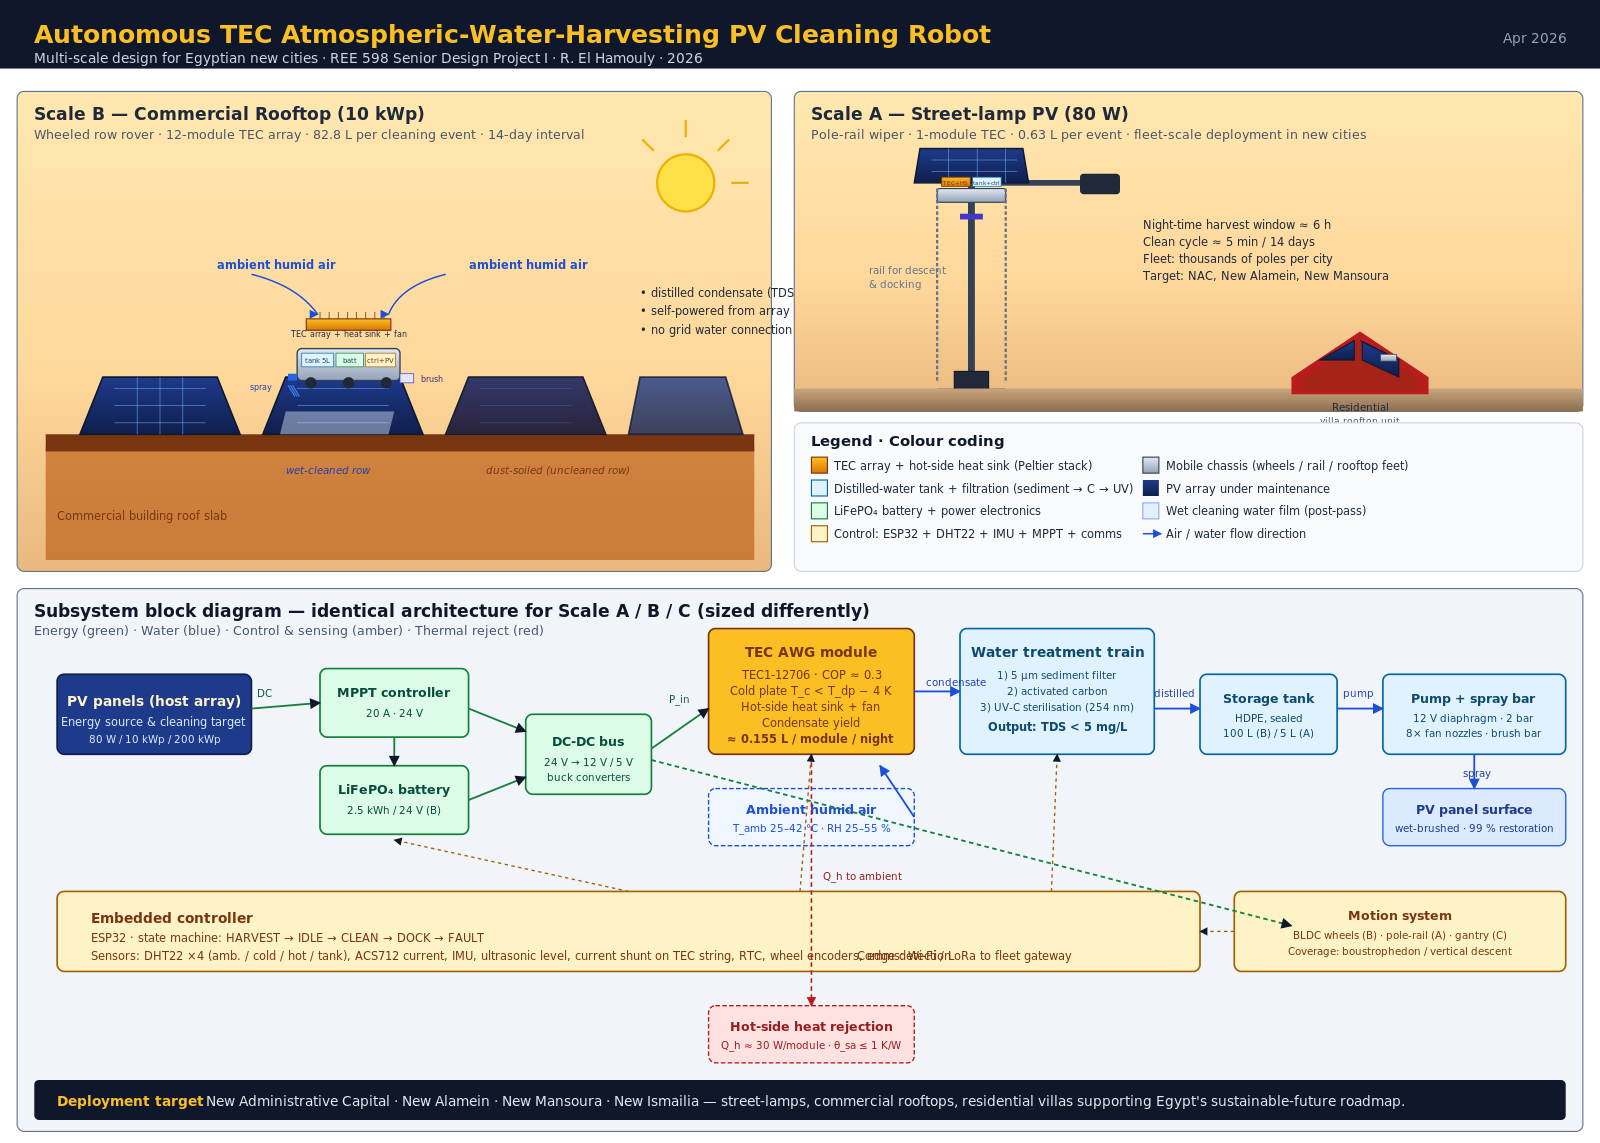
\includegraphics[width=\linewidth]{system_architecture.png}\\
      {\scriptsize Subsystem block diagram.}
    \end{column}
  \end{columns}
\end{frame}

\section{How it works}

% ===================== WATER GENERATOR =====================
\begin{frame}{The water generator: the COP vs. yield trade}
  \begin{columns}[T]
    \begin{column}{0.5\textwidth}
      \begin{itemize}\setlength\itemsep{0.4em}
        \item A coupled heat-and-mass-transfer model finds the best operating point for every hour of real climate.
        \item Push the cold side colder and you catch more water, but the efficiency (COP) drops.
        \item At the NAC the sweet spot gives \SI{38.7}{\liter\per\year} per tile, \SI{106}{\gram\per\day}, mean COP 1.91.
        \item Energy cost: about \SI{1.45}{\kWh\per\liter}.
      \end{itemize}
    \end{column}
    \begin{column}{0.5\textwidth}
      \centering
      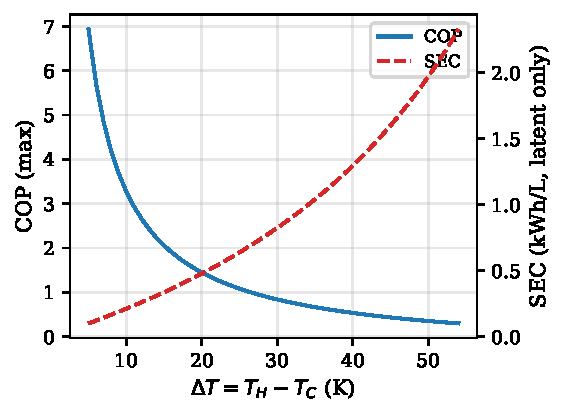
\includegraphics[width=\linewidth]{fig_cop_sec_dT.pdf}\\
      {\scriptsize COP and specific energy versus cold-side $\Delta T$.}
    \end{column}
  \end{columns}
\end{frame}

% ===================== SIZING =====================
\begin{frame}{How many tiles? The honest self-supply trade}
  The brush cleans at \SI{0.3}{\liter\per\square\meter}, so washing \SI{46}{\square\meter} of glass every 3.5 days needs only \SI{1.44}{} m$^3$/year. Full self-supply turns out to be feasible.
  \vspace{0.5em}
  \begin{center}
  \begin{tabular}{lccc}
    \toprule
    Self-supply fraction & 25\,\% & 50\,\% & 100\,\% \\
    \midrule
    TEC tiles            & 10 & 19 & \textbf{38} \\
    Energy (kWh/day)     & 1.75 & 3.25 & \textbf{6.47} \\
    Dock cost (EGP)      & 85{,}320 & 137{,}253 & \textbf{224{,}756} \\
    \bottomrule
  \end{tabular}
  \end{center}
  \vspace{0.4em}
  \begin{block}{The choice}
    100\,\% self-supply: 38 tiles at the 3.5-day schedule, about \SI{14}{\percent} of the array's own energy. Coupled to the house \SI{9.9}{\kWp} array, the marginal hardware is about \SI{14000}{} EGP.
  \end{block}
\end{frame}

% ===================== ROBOT: WHY RAIL =====================
\begin{frame}{The robot: why it ended up on rails}
  \begin{columns}[T]
    \begin{column}{0.5\textwidth}
      \textbf{The first idea did not work.} The first concept was a free-driving crawler. In simulation it could not turn on \ang{24} glass: the wheels lost traction and it slid down the slope.
      \vspace{0.5em}

      \textbf{The fix.} A rail-guided carriage. It only ever moves straight up and down the fall line, so steering on glass is no longer a problem. An \SI{8}{kg} carriage carries a full-width \SI{0.96}{m} brush.
    \end{column}
    \begin{column}{0.5\textwidth}
      \centering
      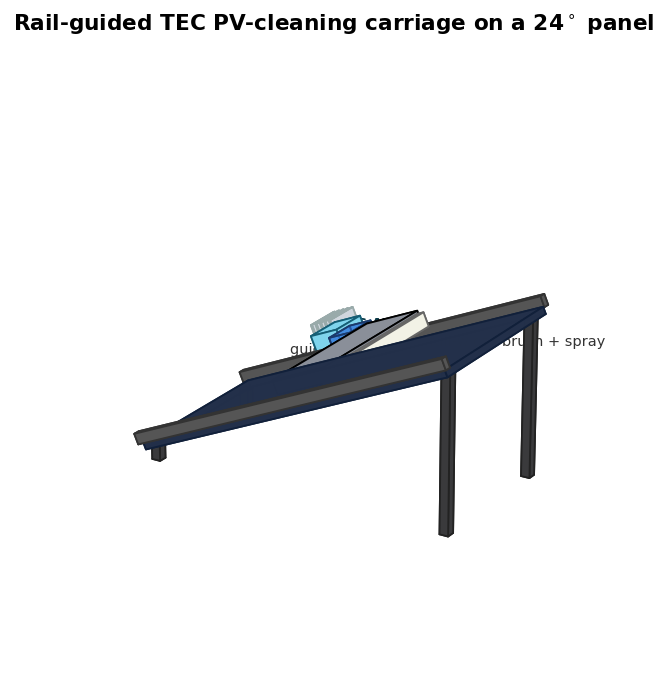
\includegraphics[width=\linewidth]{robot_3d.png}\\
      {\scriptsize Rail-guided cleaning carriage, isometric view.}
    \end{column}
  \end{columns}
\end{frame}

% ===================== CLEANING PASS =====================
\begin{frame}{One pass cleans the panel}
  \begin{columns}[T]
    \begin{column}{0.55\textwidth}
      \begin{itemize}\setlength\itemsep{0.4em}
        \item The brush is as wide as the panel, so one straight pass cleans it; no weaving side to side.
        \item Rack and pinion on both rails gives positive grip, so there is no slip on the tilt.
        \item A full down-and-up sweep takes \SI{66.7}{s} per panel, against \SI{230}{s} for the old zig-zag path.
        \item About \SI{3.6}{\liter} of water per cleaning event.
      \end{itemize}
    \end{column}
    \begin{column}{0.45\textwidth}
      \begin{block}{The geometry}
        \SI{8}{kg} carriage, \SI{0.96}{m} brush, two \SI{2.4}{m} rails, cleaning speed \SI{0.06}{\meter\per\second}.
      \end{block}
      \begin{block}{Why it is faster}
        One full-width sweep replaces six narrow passes, so a panel is clean in about a quarter of the time.
      \end{block}
    \end{column}
  \end{columns}
\end{frame}

% ===================== CONTROL =====================
\begin{frame}{The brain: two tiers and a nightly cycle}
  \begin{columns}[T]
    \begin{column}{0.52\textwidth}
      \textbf{Why two controllers}
      \begin{itemize}\small\setlength\itemsep{0.3em}
        \item A Raspberry Pi 4 runs ROS 2: the supervisor, planning, and logging.
        \item An ESP32 with micro-ROS handles the hard real-time job: PWM, encoders, and the motor PID.
        \item One chip cannot do both soft planning and tight motor loops well.
      \end{itemize}
      \vspace{0.3em}
      \textbf{No map needed.} It dead-reckons along the rails and re-registers at each panel edge.
    \end{column}
    \begin{column}{0.48\textwidth}
      \begin{block}{The cycle}
        \centering
        Idle $\rightarrow$ Harvest $\rightarrow$ Store $\rightarrow$ Clean $\rightarrow$ Dock
      \end{block}
      \begin{itemize}\small\setlength\itemsep{0.3em}
        \item Harvest and store run on cool night air; cleaning runs every 3.5 days.
        \item Safety layers gate motion on tank level and rail limits.
      \end{itemize}
    \end{column}
  \end{columns}
\end{frame}

\section{Does it work?}

% ===================== CLIMATE =====================
\begin{frame}{Climate check: the site matters a lot}
  \begin{columns}[T]
    \begin{column}{0.5\textwidth}
      \begin{itemize}\setlength\itemsep{0.4em}
        \item First validated at Benban (Aswan), the worst-case arid reference, on \num{8784} hourly records.
        \item Then re-run on the NAC rooftop (\ang{30.03} N, \ang{31.73} E) with NASA POWER hourly data.
        \item Per-tile yield rises from \SI{5.35}{\liter\per\year} at Benban to \SI{38.7}{\liter\per\year} at the NAC.
        \item That is \textbf{7.2$\times$} more water, with no dead summer month.
      \end{itemize}
    \end{column}
    \begin{column}{0.5\textwidth}
      \centering
      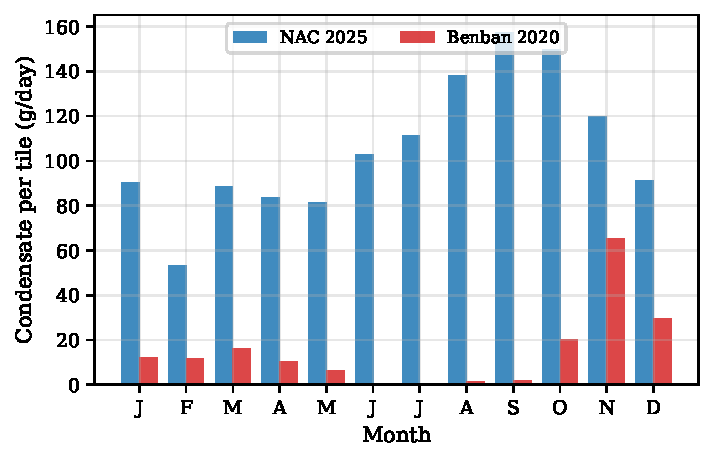
\includegraphics[width=\linewidth]{nac_monthly_water.pdf}\\
      {\scriptsize NAC monthly per-tile water yield, 2025.}
    \end{column}
  \end{columns}
\end{frame}

% ===================== SIMULATION =====================
\begin{frame}{Watching it move: the simulation}
  \begin{columns}[T]
    \begin{column}{0.5\textwidth}
      \begin{itemize}\setlength\itemsep{0.4em}
        \item Gazebo Classic 11 with ROS 2 Humble, run headless on a \ang{24} tilted panel.
        \item The free crawler lost traction and slid: the result that forced the rail design.
        \item The rail-guided carriage tracks the rails with under \SI{1}{mm} of drift and never derails.
        \item Confirms the \SI{66.7}{s} per-panel coverage used in the energy budget.
      \end{itemize}
    \end{column}
    \begin{column}{0.5\textwidth}
      \centering
      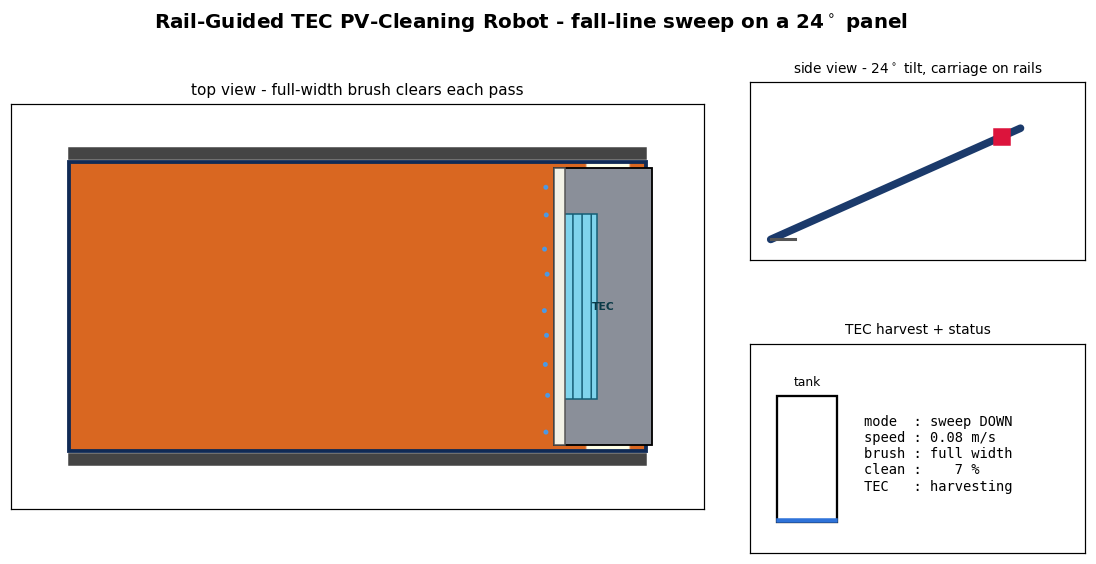
\includegraphics[width=0.78\linewidth]{sim_still_1.png}\\[0.15em]
      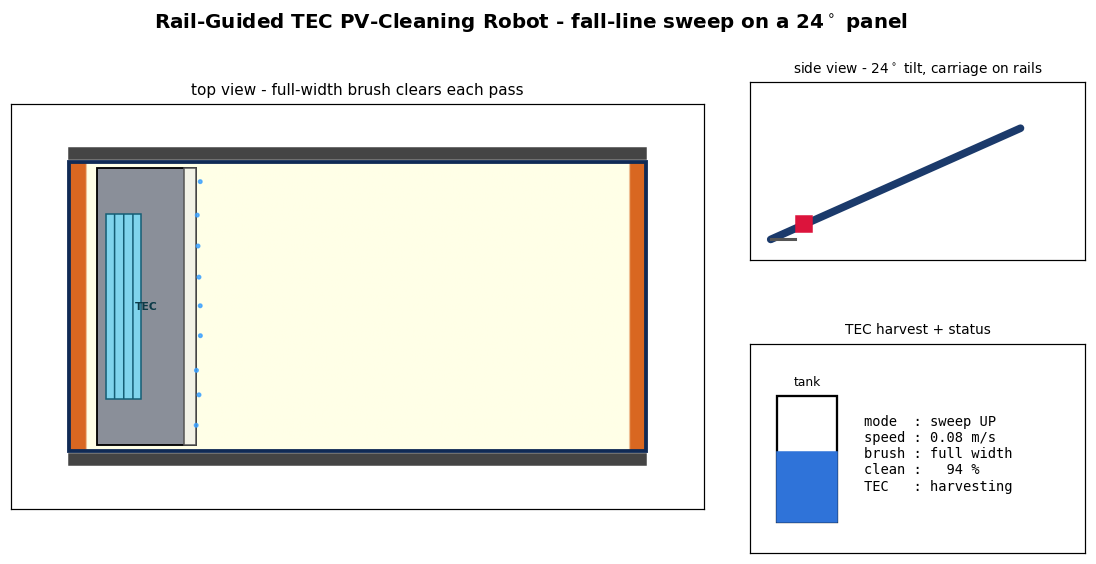
\includegraphics[width=0.78\linewidth]{sim_still_3.png}\\[0.1em]
      {\scriptsize Rail-guided sweep on the \ang{24} panel.}
    \end{column}
  \end{columns}
\end{frame}

% ===================== RESULTS =====================
\begin{frame}{Water across the whole year}
  \begin{columns}[T]
    \begin{column}{0.5\textwidth}
      \begin{itemize}\setlength\itemsep{0.4em}
        \item The 38-tile dock delivers about \SI{3.94}{\liter\per\day}, the full cleaning demand.
        \item Yield holds across all twelve months, with a summer peak and no dead season.
        \item Mean COP 1.91 over \num{3610} operating hours a year.
        \item A \SI{300}{\liter} tank smooths the month-to-month swing so the supply rarely runs dry.
      \end{itemize}
    \end{column}
    \begin{column}{0.5\textwidth}
      \centering
      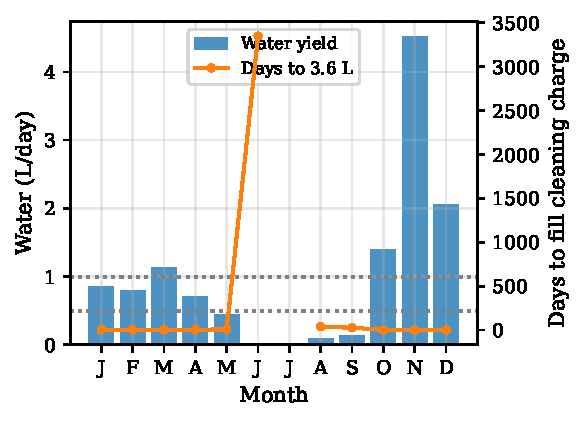
\includegraphics[width=\linewidth]{fig_monthly_water.pdf}\\
      {\scriptsize Monthly water yield across the year.}
    \end{column}
  \end{columns}
\end{frame}

\section{Building it \& why it matters}

% ===================== PROTOTYPE =====================
\begin{frame}{The bench you can build in Cairo}
  \begin{columns}[T]
    \begin{column}{0.55\textwidth}
      \textbf{Minimum bench} (about \SI{116}{} USD), every part buyable in Cairo, no imports.
      \begin{center}\small
      \begin{tabular}{lr}
        \toprule
        Block & EGP \\
        \midrule
        TEC harvesting core (4 tiles) & 2{,}110 \\
        Cleaning head (pump, brush) & 960 \\
        Sensors (DHT22, INA219, DS18B20) & 585 \\
        Control and power & 1{,}890 \\
        \midrule
        \textbf{Total} & \textbf{5{,}545} \\
        \bottomrule
      \end{tabular}
      \end{center}
    \end{column}
    \begin{column}{0.45\textwidth}
      \textbf{What the bench proves}
      \begin{itemize}\small\setlength\itemsep{0.3em}
        \item Four tiles condense measurable water in NAC-type air, logged.
        \item The pump and brush wet and sweep a soiled glass coupon.
      \end{itemize}
      \vspace{0.4em}
      \textbf{What stays in simulation}
      \begin{itemize}\small\setlength\itemsep{0.3em}
        \item The rail-guided motion (proven in Gazebo).
        \item The full dock, PV, and battery chain.
      \end{itemize}
    \end{column}
  \end{columns}
\end{frame}

% ===================== WHAT IS NEW =====================
\begin{frame}{What is new about this}
  \begin{enumerate}\setlength\itemsep{0.5em}
    \item A PV cleaner that harvests its own distilled water on site, closing the gap between dry rail robots and standalone water generators.
    \item A TEC harvesting model validated on real Egyptian climate data, with the 7.2$\times$ NAC-versus-Benban finding.
    \item An honest self-supply answer: full closure is feasible at 38 tiles, about \SI{14}{\percent} of array energy.
    \item A design pivot, crawler to rail-guided, driven by a reproducible simulation result rather than a guess.
    \item A \SI{5545}{\EGP} bench, sourced entirely in Cairo, that proves the core physics.
  \end{enumerate}
\end{frame}

% ===================== OUTRO =====================
{\setbeamertemplate{footline}{}
\begin{frame}[plain,noframenumbering]
  \begin{tikzpicture}[remember picture,overlay]
    \fill[nacblue](current page.south west)rectangle(current page.north east);
    \fill[nacteal](current page.south west)rectangle([yshift=7pt]current page.south east);
  \end{tikzpicture}
  \vfill
  \begin{center}
    {\color{nacsand}\large\bfseries The takeaway}\\[0.8em]
    {\color{white}\Large\bfseries A rooftop PV cleaner that makes its own water}\\[0.7em]
    {\color{nacteal}\rule{4cm}{2.5pt}}\\[0.8em]
    \begin{minipage}{0.82\textwidth}
      \color{white!90}\centering\small
      TEC harvesting works in Egyptian desert air, the NAC gives 7.2$\times$ the Benban yield, full self-supply needs 38 tiles at about \SI{14}{\percent} of array energy, the motion is validated in Gazebo, and the physics is provable on a \SI{5545}{\EGP} Cairo bench.
    \end{minipage}\\[1.4em]
    {\color{white}\large\bfseries Thank you for watching}\\[0.3em]
    {\color{white!75}\small Rahma El-Hamouly \quad{\textbullet}\quad REE\,598}
  \end{center}
  \vfill
\end{frame}}

\end{document}
